\documentclass[a4paper]{book}
\usepackage[utf8]{inputenc}
\usepackage{cite}
\bibliographystyle{acm}
\usepackage{amsmath}
\usepackage{amsfonts}
\usepackage{graphicx}
\usepackage{amssymb}
\usepackage{caption}
\usepackage{lipsum}
\usepackage{multirow}
\author{César Lozano. Departamento de Química Farmacéutica y Orgánica.}
\title{\textbf{Cuaderno de laboratorio.}\\ Obtención de nuevas drogas sintéticas en la cocina de tu casa. El primer paso hacia tu propia red de narcotráfico}


\begin{document}

\maketitle

\thispagestyle{empty}
$\ $

\tableofcontents

\pagenumbering{arabic}
\setcounter{page}{150}

\chapter{CLL152}
\begin{center}
\begin{huge}
Primera reacción que tienes que hacer para forrarte
\footnote{Empieza en la página 150 porque es la continuación del un primer libro titulado: Ganarte la vida de forma ilegal.}
\end{huge}
\end{center}

\begin{large}
\textbf{Método de la reacción} \\
\end{large}
\\
En la olla donde te haces los macarrones echamos el producto 1 (200 miligramos, si queréis ganar más dinero echad más) y luego el producto 2. Al final echamos el agua y si tienes gas lo dejas media hora, si tienes vitro 1 hora a medio fuego.
\\
Al final se forman cristales y eso es lo bueno \cite{2}.
\\
Para calcular el agua que tenemos que echar seguimos la siguiente fórmula:
\begin{equation}
\int = \dfrac{\oint^2_3}{dX}
\end{equation}


\begin{large}
\textbf{Reactivos} 
\end{large}
\begin{table}[htb]
\centering
\begin{tabular}{|c|c|c|c|c|c|}
\hline 
\multirow{2}{1.5cm}{Producto 1} & \textbf{Masa} & \textbf{Ml} & \textbf{Moles} & \textbf{Mmoles} & \textbf{Equivalentes} \\ \cline{2-6} 
& 200 mg & - & 0.0019031 & 1.9031 & 1 \\ 
\hline 
• & • & • & • & • & • \\ 
\hline 
• & • & • & • & • & • \\ 
\hline 
• & • & • & • & • & • \\ 
\hline 
• & • & • & • & • & • \\ 
\hline 
\end{tabular} 
\end{table}

\begin{table}[hbt]
\begin{center}
\begin{tabular}{|c|c|c|c|}
\hline
\textbf{Disolvente} & \textbf{Ml} & \textbf{Mmoles} & \textbf{Ml/Mmoles} \\
\hline
- & - & - & - \\
\hline
\end{tabular}
\end{center}
\end{table}

\newpage
\begin{large}
\textbf{Producto Final}
\footnote{Pruebas necesarias para comprobar que el producto obtenido está bien, aunque como lo hacemos en la cocina va a ser complicado hacerlas la verdad...}\\
\end{large}
\begin{enumerate}
\item Peso Molecular:
\item Rendimiento:
\item Punto de Fusión:
\item Protón:
\item Carbono:
\item DEPT:
\item Masas:
\item Muestra:
\end{enumerate}


\begin{center}
\begin{figure}[hbt]
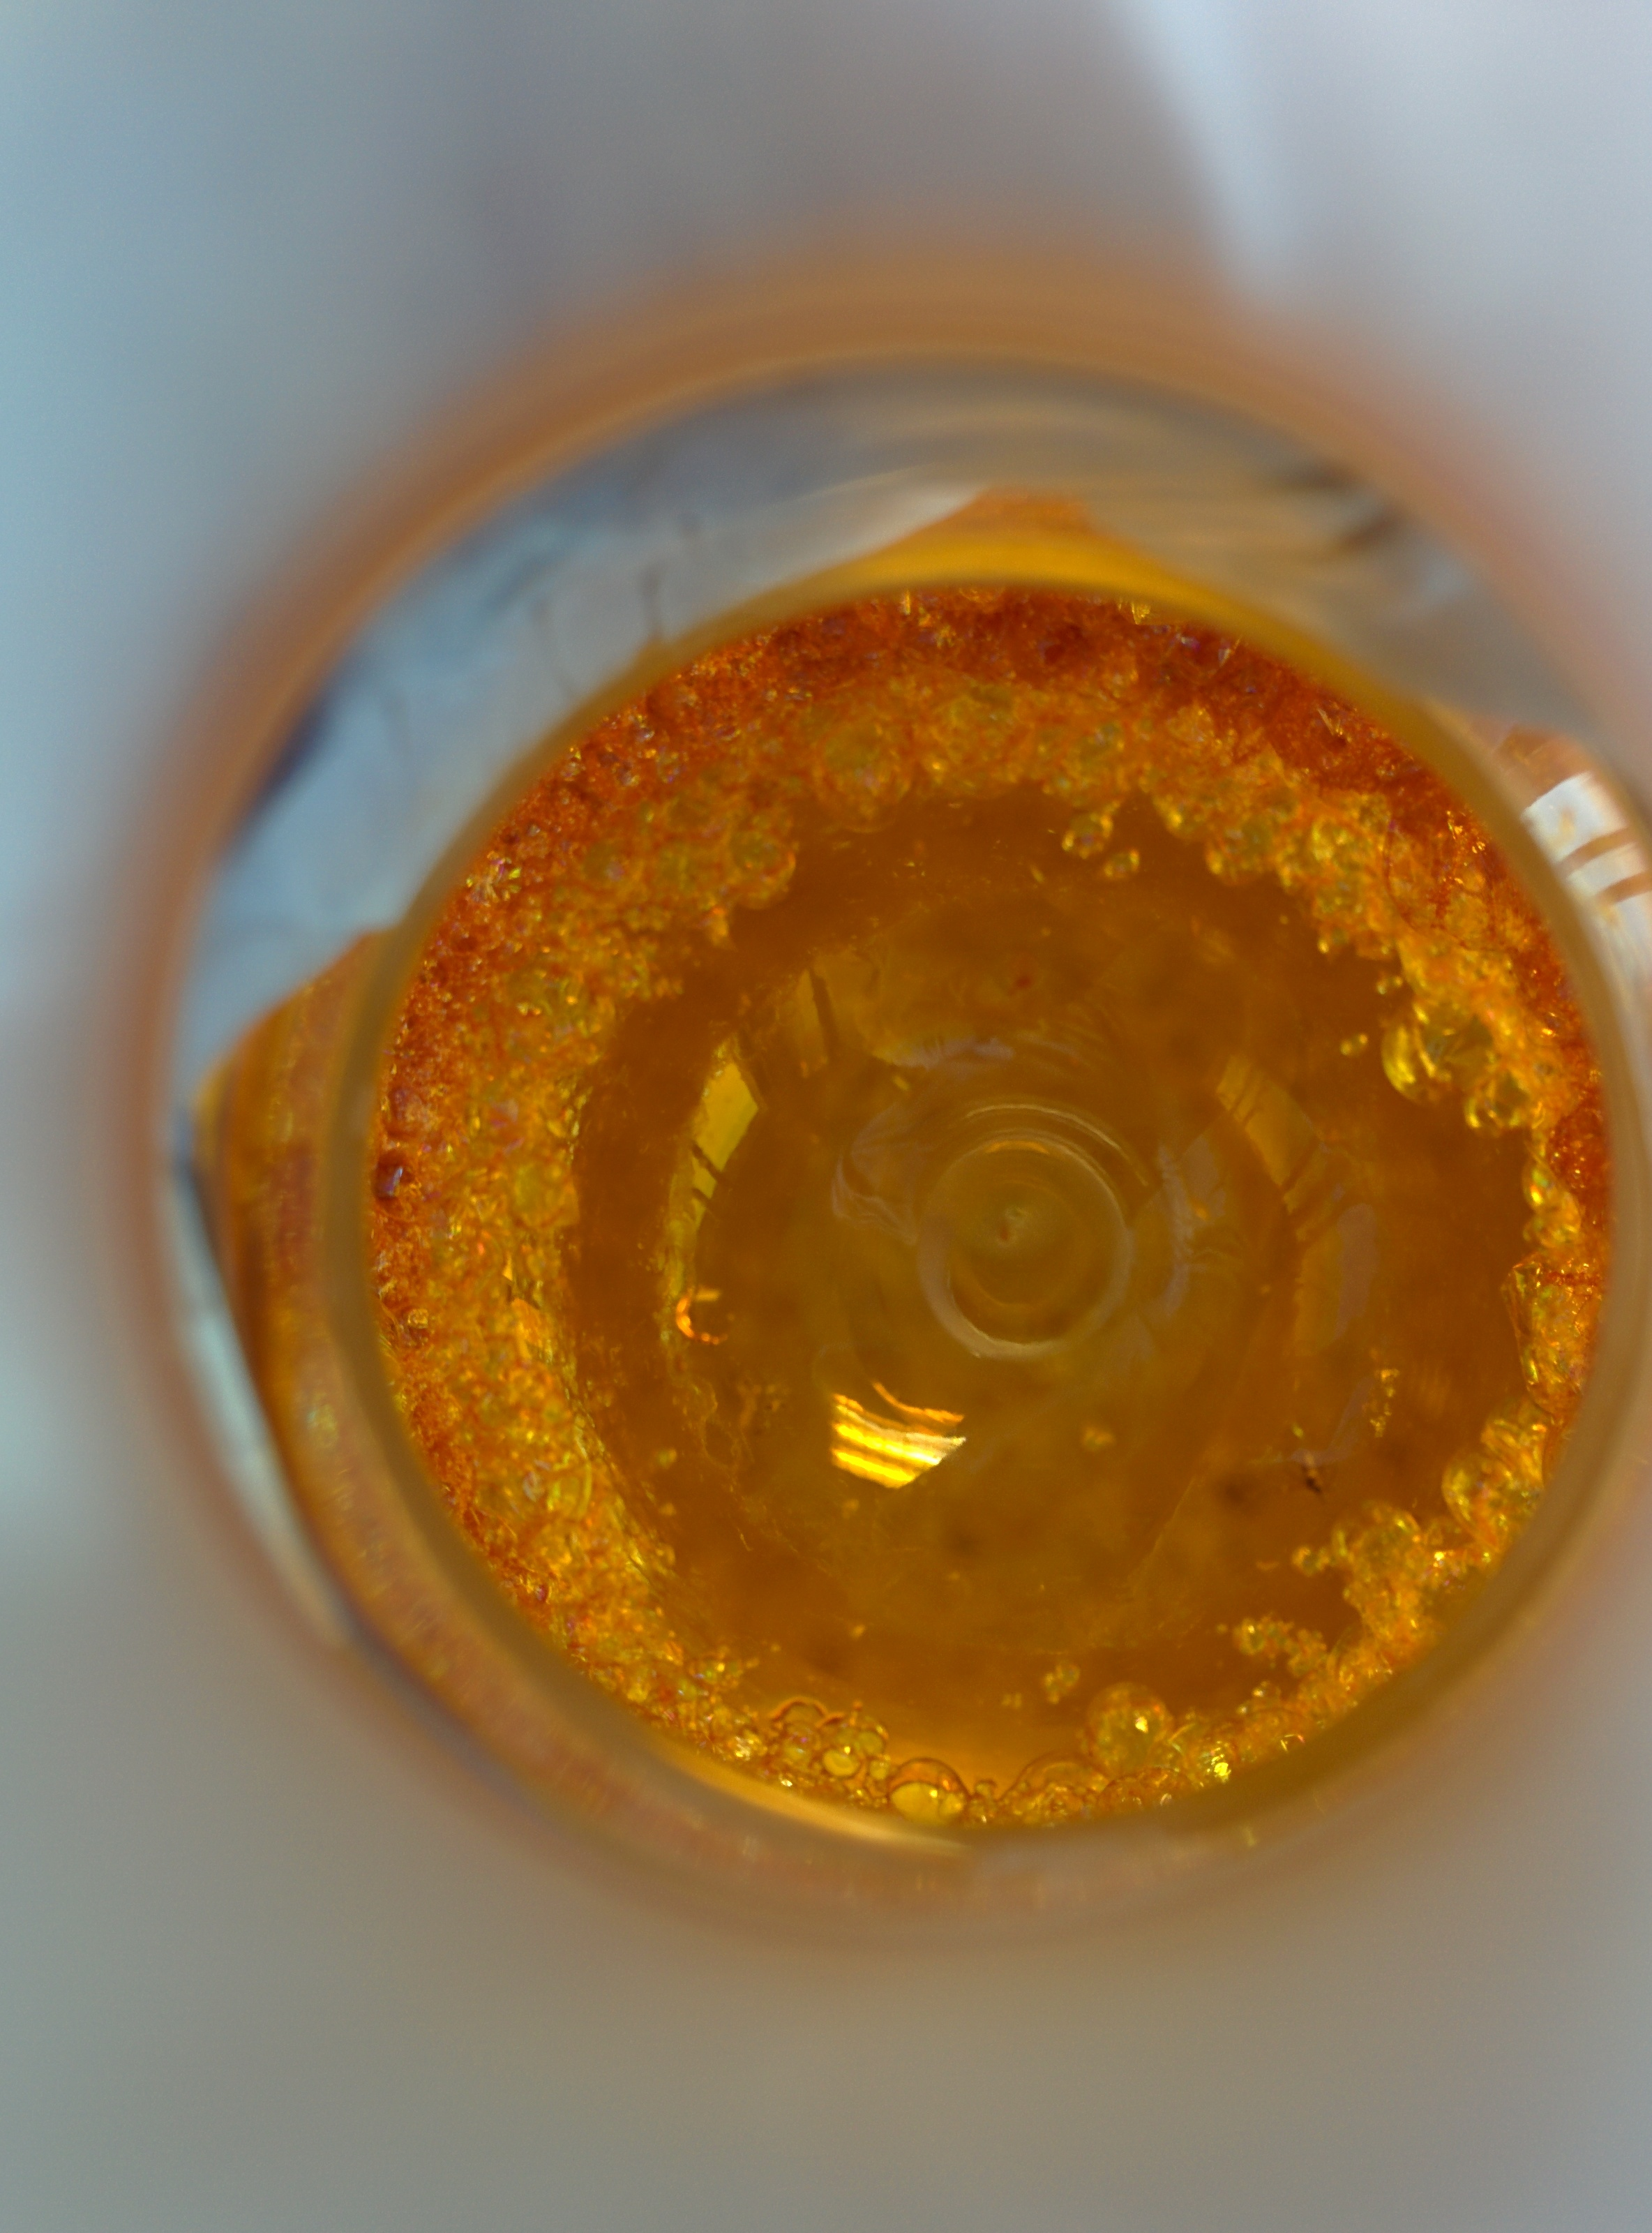
\includegraphics[scale=0.07]{./1.jpg}
\caption{Así debe de quedar la reacción\textcopyright}
\end{figure}
\end{center}

\newpage

\cleardoublepage

\bibliography{citas}

\end{document}

